\subsection*{Introduction}


De nos jours, la \emph{Vision par ordinateur} et le \emph{traitement d'images (PI)} sont omniprésents dans la vie
quotidienne des gens. Ils sont présents à chaque fois que nous passons devant une caméra de vidéosurveillance, à chaque
fois que nous allons à l'hôpital faire une IRM, à chaque fois que nous conduisons notre voiture et passons devant un
radar et à chaque fois que nous utilisons notre ordinateur, smartphone ou tablette. Ils sont devenu incontournables. Les systèmes utilisant cette technologie sont parfois simples et parfois plus complexes. Aussi, l'usage qui est fait de
cette technologie a de nombreuses finalités telles que l'observation spatiale, l'imagerie médicale, l'amélioration de la
qualité de vie, la surveillance, le contrôle, les systèmes autonomes, etc. Désormais, le \emph{traitement d'images}
dispose d'un large éventail de sujets de recherche et malgré une masse de travaux antérieurs déjà contribués très
importante, il reste encore beaucoup à explorer.

Prenons l'exemple d'une application smartphone moderne qui propose une reconnaissance faciale afin de reconnaître les
personnes qui figurent dans d'une photo. Pour fournir un résultat précis, cette application devra faire beaucoup de
traitements différents en plusieurs étapes. De plus, il y a beaucoup de variables à gérer. Nous pouvons énumérer (non
exhaustivement) la météo, l'exposition lumineuse, la résolution, l'orientation, le nombre de personnes, la localisation
de la personne, la distinction entre les humains et les objets/animaux, etc. Tous ces éléments doivent être
soigneusement gérés afin de reconnaître enfin la ou les personne(s) figurant dans la photo. Ce que l'application ne vous
dit pas, c'est la complexité de la pipeline de traitement d'images en coulisse  qui, la plupart du temps, ne peut même
pas être exécuté dans son intégralité sur son appareil (smartphone, tablette, \ldots). En effet, le traitement d'images
est coûteux en ressources informatiques et ne répondrait pas à la contrainte de temps demandée par l'utilisateur si
l'intégralité de la pipeline était exécutée sur l'appareil. Par ailleurs, pour la dernière partie qui est de <<
reconnaître la personne sur la photo >>, l'application doit alimenter la photo pré-traitée à un réseau de neurones formé
au préalable par des techniques d'apprentissage en profondeur afin de donner une réponse précise. Il existe des
technologies capables d'intégrer un réseau de neurones dans un téléphone mobile, telles que
MobileNets~\parencite{howard.2017.mobilenets}, mais il reste limité en termes de capacités opérationnelles. Il peut
détecter un être humain à l'intérieur d'une photo, mais ne peut pas dire qui est cet être humain par exemple. C'est
pourquoi les systèmes de réseau de neurones précis sont généralement hébergés dans le cloud, ce qui ne les rend
disponibles que via Internet. Lors du téléchargement de son image, l'utilisateur n'imagine pas la quantité de
technologies et de puissance de calcul qui va être utilisée pour trouver la personne apparaissant sur la photo.

Nous comprenons maintenant que, de nos jours, pour créer des applications qui interagissent avec des photos ou des
vidéos, nous devons pouvoir effectuer un traitement d'images précis, rapide et évolutif sur une multitude d'appareils
(smartphone, tablette, \ldots). Afin d'atteindre cet objectif, les traiteurs d'image doivent disposer de deux types
d'outils. Le premier est l'environnement de prototypage, une boîte à outils qui permet au traiteur d'image de
développer, tester et améliorer sa logique applicative. Le second est l'environnement de production qui déploie la
version viable de l'application qui a été développée par le traiteur d'image. Les deux environnements peuvent ne pas
avoir les mêmes besoins. D'une part, l'environnement de prototypage nécessite généralement de disposer d'une boucle de
rétroaction rapide pour les tests et d'une disponibilité des algorithmes des logiciels existants à la pointe des
connaissances actuelles. De cette façon, le traiteur d'image peut facilement construire ses nombreux prototypes
par-dessus ces briques de base (algorithmes existants) pour obtenir des résultats rapidement dans le but de pouvoir
itérer de manière agile. D'autre part, l'environnement de production doit, quant à lui, être stable, résilient, rapide
et évolutif.

Lorsque l'on regarde les standards de l'industrie aujourd'hui, nous remarquons que le langage de programmation
\emph{Python} est le principal choix pour le prototypage. Cependant, Python peut ne pas convenir pour pouvoir déployer
un prototype viable en production avec un minimum changements par la suite. Nous trouvons qu'il n'est pas idéal que le
traiteur d'image ne puisse pas profiter de nombreuses opportunités d'optimisations, à la fois en termes d'efficacité
algorithmique et à la fois au niveau d'une meilleure utilisation du matériel. Il serait beaucoup plus efficace d'avoir
des blocs de construction de base de bas niveau qui pourraient être adaptés pour convenir à autant de cas d'utilisation
que possible. De cette façon, le traiteur d'image pourrait facilement s'appuyer sur ces blocs lors de la conception de
son application. Nous distinguons deux types de cas d'utilisation. Le premier concerne la multiplicité des types ou des
algorithmes auxquels le traiteur d'image est confronté. Le deuxième relève de la diversité du matériel sur lequel il
peut vouloir exécuter son programme. L'objectif est d'avoir des blocs de construction qui peuvent être suffisamment
intelligents pour tirer parti des nombreuses opportunités d'optimisation, tant en ce qui concerne les types de données
et d'algorithmes en entrée, que le matériel cible. Ensuite, le traiteur d'image verrait une importante amélioration des
performances, par défaut, sans devoir ajuster spécifiquement son application. C'est ainsi que le concept de généricité
est introduit. Il vise à fournir un terrain d'entente sur la façon dont une image doit se comporter lorsqu'elle est
transmise à des algorithmes de base nécessaires pour des applications complexes. De cette façon, en théorie, il suffit
d'écrire l'algorithme une seule fois pour qu'il fonctionne avec n'importe quel type d'image.

Finalement, il est admis qu'il existe une règle concernant les trois points suivants : la généricité, l'efficacité et la
facilité d'utilisation. La règle énonce que l'on ne peut avoir que deux de ces avantages qu'en sacrifiant le troisième.
Si l'on veut être générique et efficace, alors la solution naïve sera très complexe à utiliser avec beaucoup de
paramètres. Si l'on veut qu'une solution soit générique et facile à utiliser, alors elle ne sera pas très efficace par
défaut. Enfin, si l'on souhaite qu'une solution soit simple d'utilisation et efficace alors elle ne sera pas très
générique. Pour illustrer cette règle, nous pouvons trouver des exemples parmi les bibliothèques existantes. Une
bibliothèque notablement générique et efficace en C++ est Boost~\parencite{boost.2021} : elle est également notoirement
connue pour être difficile à utiliser. Les composants tels que Boost.Graph, Boost.Fusion ou Boost.Spirit sont difficiles
à utiliser. Aussi, une bibliothèque qui est générique et facile à utiliser est le parser Json écrit par Niels
Lohmann~\parencite{nlohmann.2021.json}. Il s'efforce de gérer chaque cas d'utilisation tout en restant très simple à
intégrer et à utiliser côté code utilisateur (syntaxe très proche du Json natif en code C++ en fournissant un DSL
(Domain Specific Language)~\parencite{deursen.2000.DSL} pour convertir directement les structures C++ en donnée Json).
Cependant, cela a un coût et ce parser est plus lent qu'un parser Json optimisé pour la performance tel que
simdjson~\parencite{lemire.2021.simdjson} dont le but est de << parser des gigaoctets de JSON par seconde >>. Enfin, il
existe de nombreux exemples de code convivial et efficace qui ne sont pas génériques. Nous pouvons citer
Scikit-image~\parencite{vanderwalt.2014.skimage} et OpenCV~\parencite{bradski.2000.opencv}, faciles à utiliser et
efficace (beaucoup de code SIMD/GPU manuscrit) mais pas générique en raison des choix de conception.

Dans cette thèse, nous avons choisi de travailler sur une bibliothèque de traitement d'images en poursuivant les travaux
sur Pylene~\parencite{carlinet.2018.pylena}. Mais travailler uniquement au niveau de la bibliothèque restreindrait
l'utilisabilité de notre travail et donc son impact. C'est pourquoi nous visons à toucher les utilisateurs mettant au
point des prototypes en fournissant un package qui peut être utilisé par un langage dynamique tel que Python, sans
sacrifier les performances. En particulier, nous visons la disponibilité d'utilisation dans un notebook Jupyter. Un
objectif très important pour nous est d'être utilisable en milieu éducatif, ce qui est une force de Python. Dans cette
bibliothèque, nous montrons comment être générique et performant, tout en restant facile à utiliser. Ce faisant, nous
nous efforçons de casser la règle citée précédemment. Le périmètre de la bibliothèque se limite à la morphologie
mathématique~\parencite{najman.2013.mathematical,geraud.2010.book} et la fourniture de types d'image versatiles. Nous
tirons parti du langage C++ moderne et de ses nombreuses nouvelles fonctionnalités liées à la généricité et à la
performance pour dépasser cette règle dans la zone de traitement d'images. Enfin, nous tentons, d'apporter les outils et
les concepts de bas niveau du monde statique au monde du prototypage de haut niveau et dynamique pour une meilleure
diffusion et facilité d'utilisation, grâce un pont entre ces deux mondes.

C'est avec cette philosophie à l'esprit que ce manuscrit présente notre travail de thèse lié au langage C++ appliqué au
traitement d'images. Il est organisé comme suit :

\paragraph{Programmation générique (généricité)} Ce chapitre présente l'état de l'art sur la notion de généricité. Nous
expliquons son origine, comment il a évolué au fil du temps (en particulier dans le langage C++), quels problèmes il
résout et quels problèmes il crée. Nous expliquons pourquoi le traitement d'images et la généricité fonctionnent bien
ensemble. Enfin, nous faisons le tour des outils existants qui permettent à la généricité (intrinsèquement restreinte au
langage compilé) d'exister dans le monde dynamique (avec langages interprétés tels que Python).

\paragraph{Taxonomie pour le traitement d'images : types d'image et algorithmes.} Ce chapitre présente notre première
contribution dans le domaine du traitement d'images qui consiste à réaliser une taxonomie complète des différentes
familles d'images ainsi que des différentes familles d'algorithmes. Ce chapitre explique, entre autres, la notion de
concept et son application au domaine du traitement d'images. Nous expliquons comment extraire un concept d'un code
existant et comment l'exploiter pour le rendre plus efficace et plus lisible. Nous proposons enfin notre point de vue
sous la forme d'une collection de concepts liés au domaine du traitement d'images.

\paragraph{Les Vues d'Image} Ce chapitre présente notre deuxième contribution qui est une généralisation du concept de
Vues (tiré du langage C++, du travail sur les \emph{ranges}~\parencite{niebler.2018.ranges}) aux images. Cela permet la
création d'images légères et peu coûteuses à copier. Cela permet également d'avoir une approche beaucoup plus simple
pour concevoir une pipeline de traitement d'images en enchaînant les opérations directement dans le code de manière
intuitive. Les \emph{ranges} sont le ciment d'une nouvelle façon de designer des algorithmes pour faciliter
l'utilisation des images, ce qui améliore donc leur aspect générique. Enfin, nous discutons du concept d'évaluation
paresseuse et de l'impact des vues sur les performances.

\paragraph{Un pont entre le monde statique et le monde dynamique} Ce chapitre présente notre troisième contribution qui
est un moyen de donner accès aux fonctionnalités génériques d'un langage compilé (tel que C++) à un langage dynamique
(tel que Python) pour faciliter le passage entre la phase de prototypage et la phase de production. En effet, pour
parvenir à une communication efficace entre le code dynamique et le binaire de la bibliothèque statique, il faut être en
mesure de concilier du code C++ générique dont la généricité est résolue au moment de la compilation (ce que nous
appelons le << monde statique >>), et du code Python dynamique qui s'appuie sur des packages binaires pré-compilés (ce
que nous appelons le << monde dynamique >>) : et cela n'est vraiment pas évident. D'autant plus que nous ne pouvons pas
non plus exiger de l'utilisateur qu'il fournisse et utilise un compilateur à chaque fois qu'il veut utiliser notre
bibliothèque depuis Python. Dans ce chapitre, nous discutons quelles sont les solutions existantes qui peuvent être
envisagées ainsi que leurs avantages et inconvénients. Nous discutons ensuite de la manière dont nous avons conçu et
réalisé une solution hybride pour arriver à faire ce pont entre le monde statique et le monde dynamique.


\subsection*{Programmation générique (généricité)}


En langage naturel, quelque chose est générique quand il peut répondre à plusieurs objectifs à la fois, tout en étant un
minimum efficace. Par exemple, un ordinateur est un outil générique qui permet de rédiger des documents, d'accéder à des
e-mails, de parcourir Internet, de jouer à des jeux vidéo, de regarder des films, de lire des e-books etc. En
programmation, un outil est dit générique lorsqu'il peut répondre à plusieurs objectifs. Par exemple, le compilateur gcc
peut compiler plusieurs langages de programmation (C, C++, Objective-C, Objective-C++, Fortran, Ada, D, Go et BRIG
(HSAIL)) ainsi que cibler plusieurs architectures (IA-32 (x86), x86--64, ARM, SPARC, etc.). Désormais, on peut dire que
gcc est un compilateur générique. À ce stade, il est important de noter que même si un outil est considéré comme
générique, il y a une limitation quant à ce que cet outil peut faire et ce qu'il ne peut pas faire. Un compilateur
malgré la prise en charge de nombreuses langues et architectures, ne pourra pas passer un appel téléphonique ou faire un
café. De ce fait, il est important de noter que la généricité est un aspect qui qualifie quelque chose. Dans ce
chapitre, nous étudions les aspects génériques liés aux bibliothèques et aux langages de programmation.

Cette thèse volontaire laisse de côté l'aspect générique lié à l'architecture cible. En effet, savoir écrire et/ou
générer du code capable de s'exécuter sur un large éventail d'architectures matérielles différentes est un domaine de
recherche à lui tout seul et n'est pas l'objet principal de cette thèse. Il est également connu sous le nom de
\emph{informatique hétérogène}. Au lieu de cela, nous allons nous concentrer sur les aspects liés à la généricité au
niveau de la bibliothèque et au niveau du langage de programmation.

\paragraph{Généricité au sein des bibliothèques} Elle est décrite par la cardinalité du nombre de cas d'utilisation
qu'elle peut gérer. Les bibliothèques fournissent toujours leurs propres structures de données, pour représenter et
donner un sens aux données que l'utilisateur veut traiter, ainsi que des algorithmes pour traiter ces données et fournir
différents types de résultats. Une bibliothèque sera alors cataloguée comme
\emph{générique}~\parencite{musser.1994.algorithm} lorsque (i) ses structures de données permettent à l'utilisateur de
s'exprimer entièrement, sans limitation et lorsque (ii) sa banque d'algorithmes est suffisamment grande pour faire tout
ce que l'utilisateur voudrait faire avec ses données. En réalité, une telle bibliothèque n'existe pas et il y a toujours
des limitations. Étudier ces limites et quelles raisons les motivent est la clé pour comprendre comment les dépasser à
l'avenir, en développant le support de nouveaux matériels et/ou logiciels pour de nouvelles fonctionnalités permettant
plus de généricité.

\paragraph{Généricité dans les langages de programmation} Elle est décrite par la capacité du langage à exécuter le même
code sur une grande quantité de structures de données~\parencite{dehnert.1998.fundamentals}, qu'elles soient natives
(char, int, \ldots) ou définies par l'utilisateur. Il est aujourd'hui primordial qu'un langage de programmation puisse
le faire. En effet, dans un monde où les technologies de l'information sont omniprésentes, la quantité de code écrit par
les développeurs de logiciels est faramineuse. Et il en va de même pour la quantité de bogues et de vulnérabilités de
sécurité. Pouvoir avoir nativement un langage de programmation qui permet de faire \emph{plus} en écrivant \emph{moins}
se traduit mathématiquement par un coût de développement et de maintenance réduit. Les langages de programmation offrent
de nombreuses façons d'atteindre la généricité qui dépendent des spécificités intrinsèques des langages : compilés ou
interprétés, natifs ou émulés, etc.

Avant d'entrer dans les détails de ce que la généricité implique pour les bibliothèques et les langages de
programmation, il est nécessaire d'introduire un peu de vocabulaire. Le premier terme est la notion de \emph{type}. Un
\emph{type} (ou \emph{type de données}) est un attribut de données qui indique au compilateur ou à l'interpréteur
comment le programmeur a l'intention d'utiliser les données. La grande majorité des langages de programmation prend en
charge les types de données de base (également appelés types primitifs) tels que les nombres entiers, les nombres à
virgules flottantes, les types booléens et les chaînes de caractères (ASCII, Unicode, etc.). Cet attribut de type
définit les opérations qui peuvent être effectuées sur les données, la signification des données ainsi que la taille des
données en mémoire (les données peuvent alors être stockées sur le tas, la pile, etc.). Un type de données fournit un
ensemble de valeurs à partir desquelles une expression (c'est à dire variable, fonction, etc.) peut prendre ces valeurs.
Parmi les langages de programmation, nous pouvons distinguer ceux qui sont dynamiquement typés et ceux qui sont
statiquement typés. Les langages typés statiquement sont ceux dont les variables sont déclarées contenant un type
spécifique. Cette variable ne peut contenir des données d'un autre type dans le champ où elle est déclarée. Des langages
de programmation à typage statique sont Ada, C, C++, Java, Rust, Go et Scala. Les langages typés dynamiquement sont ceux
dont les variables peuvent être réassignées avec une valeur de type différent de celui avec lequel elle a été
initialement déclarée. Le type de variable est ensuite modifié dynamiquement pour s'adapter à la nouvelle valeur qu'elle
porte. Des langages de programmation à typage dynamique sont PHP, Python, JavaScript et Perl.

La conséquence de pouvoir dire quel type une variable contient à tout moment (langage à typage statique) est double.
Pour le développeur, il est plus facile de raisonner sur le code et de repérer les bugs. Pour le compilateur, il est
possible de générer un code binaire optimisé spécifiquement pour ce type de données (vectorisation, etc.). La
conséquence de pouvoir transformer le type qu'une variable peut contenir au moment de l'exécution sert principalement à
faciliter le prototypage. Lors de la modification d'un notebook Jupyter, il est très apprécié de ne pas se limiter à un
seul type pour chaque variable déclarée afin de pouvoir itérer sur le prototype plus rapidement.

En traitement d'images, une image \(Im\) est définie sur un domaine \(\mathcal{D}\) (qui contient des points) par la
relation \(\forall x \in \mathcal{D}, y = Im(x)\) où \(y\) est la valeur de l'image \(Im\) pour le point \(x\). Cette
définition se traduit toujours par une structure de données complexe lorsqu'elle est transposée dans un langage de
programmation. Cette structure de données doit connaître la mémoire tampon contenant les données de l'image
ainsi que des informations sur la taille et les dimensions de l'image. De plus, ajoutant à la difficulté, les
informations nécessaires pour définir précisément la structure des données ne sont pas toujours connues lors de
l'écriture du code source. En effet, un cas d'utilisation très simple consiste à lire une image dans un fichier pour la
charger en mémoire. Le fichier peut contenir une image de différents types de données et le programme doit toujours
fonctionner correctement. Il y a de multiples approches pour résoudre ce problème, et nous les abordons dans ce
chapitre.

En projetant la notion de généricité au traitement d'images, nous pouvons déduire que nous avons besoin de deux aspects
importants pour être générique. Tout d'abord, nous devons décorréler les structures de données de leur topologie et des
données sous-jacentes des algorithmes. En effet, nous voulons que nos algorithmes supportent autant de structures de
données que possible. Ensuite, nous pouvons factorisés ensemble de nombreux algorithmes partageant le même schéma
calculatoire.

\begin{figure}[htbp]
  \centering
  \begin{tabular}{cccc}
                                                                           & image 2D
                                                                           & graphe   & maillage \\[5pt]
    entrée:                                                                &
    \fbox{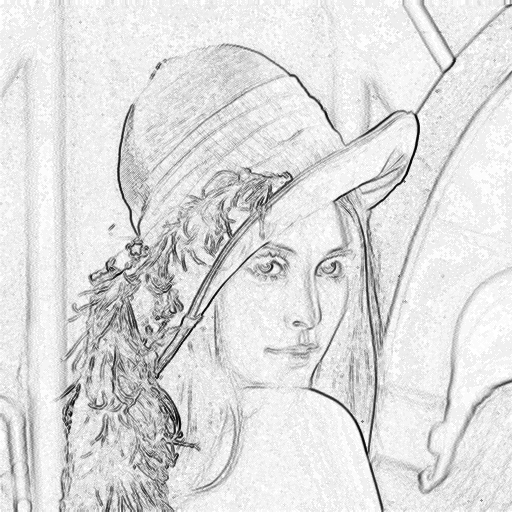
\includegraphics[width=.2\linewidth]{../figures/geninput-000b}}  &
    \fbox{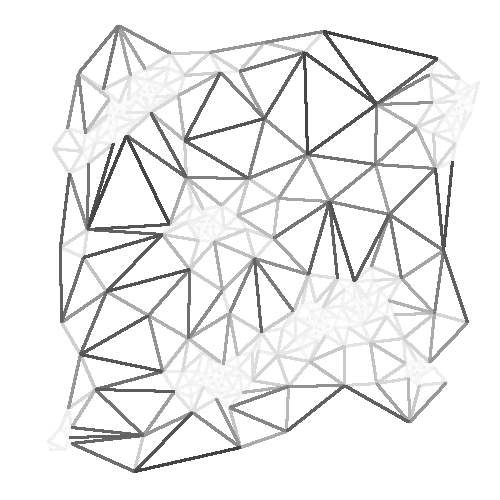
\includegraphics[width=.2\linewidth]{../figures/geninput-001b}}  &
    \fbox{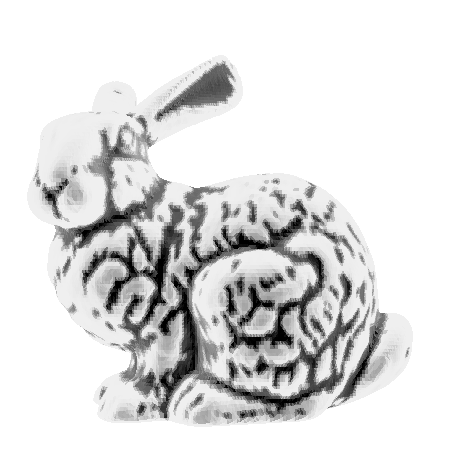
\includegraphics[width=.2\linewidth]{../figures/geninput-002b}}
    \\[5pt]
    %
    sortie:                                                                &
    \fbox{
\includegraphics[width=.2\linewidth]{../figures/genoutput-000}}  &
    \fbox{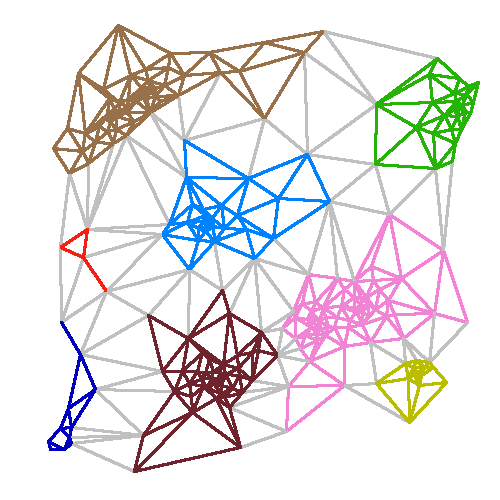
\includegraphics[width=.2\linewidth]{../figures/genoutput-001b}} &
    \fbox{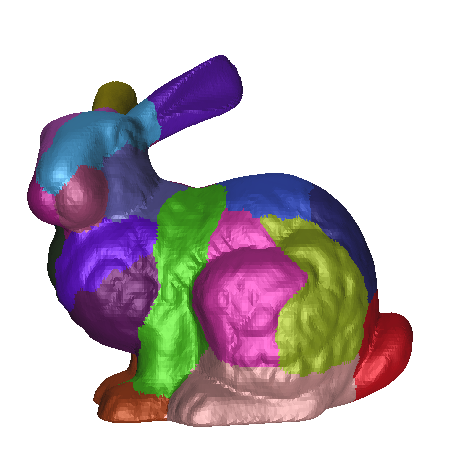
\includegraphics[width=.2\linewidth]{../figures/genoutput-002b}}
    \\
  \end{tabular}
  \bigskip

  \text{Le même code tourne sur toutes ces différentes données d'entrée.}

  \caption[]{Algorithme de ligne de partage des eaux appliqué à trois types d'image différents.}
  \label{resume:fig:type.vs.algo}
\end{figure}

La généricité peut avoir deux significations différentes selon les personnes que vous interrogez. Par exemple, certaines
diront que la généricité est un aspect haut niveau et vont qualifier un outil comme étant << suffisamment générique >>
lorsque celui-ci peut gérer tous ses cas d'utilisation. D'autres soutiendront que la généricité est un aspect bas niveau
et va donc concerner la machine fabriquant l'outils (code), << suffisamment générique >> pour fabriquer toutes sorte
d'outils. Ni l'un ni l'autre n'a tort. Cependant, pour des raisons de compréhension, nous utiliserons des mots
différents pour chacun de ces cas. Un outil assez générique pour gérer un grand nombre de cas d'utilisation sera appelé
\emph{versatile}. Enfin, pour un outil dont le but est de fournir un environnement de programmation capable de gérer
le code de n'importe quel cas d'utilisation, nous utiliserons le terme \emph{généric}. Dans cette thèse, la généricité
concernera le code. La~\cref{resume:fig:type.vs.algo} illustre le résultat d'une même implémentation générique de
l'algorithme de ligne de partage des eaux, qu'il soit appliqué sur une image 2D, un graphe ou un maillage.

Dans ce chapitre nous présentons l'origine de la programmation générique, qui remonte à
l'année~\citedate[year]{musser.1988.generic} et comment elle a évolué pour être intégrée dans le langage de
programmation Ada puis dans le langage de programmation C++. Son évolution s'est poursuivie avec l'arrivée de la notion
de \emph{concept} qui complétera la boîte à outils nécessaire pour pouvoir pleinement utiliser la programmation
générique sans recourir à des techniques et outils obscurs.

\begin{table}[htbp]
  \centering
  \begin{threeparttable}
    \caption[]{Approches de la généricité : avantages ~\& inconvénients}
    \begin{tabular}[width=0.8\linewidth]{l|ccccc}
      Paradigme                     & VT\tnote{1} & SC\tnote{2} & E\tnote{3} & Une IA\tnote{4} & AE\tnote{5} \\
      \hline
      Duplication de Code           & \cmark      & \xmark      & \cmark     & \xmark          & \xmark      \\
      Généralisation de Code        & \xmark      & \eqmark     & \eqmark    & \cmark          & \xmark      \\
      Programmation Orientée Object & \eqmark     & \cmark      & \xmark     & \cmark          & \cmark      \\
      Programmation Générique:      &             &             &            &                 &             \\
      \quad avec C++11              & \cmark      & \eqmark     & \cmark     & \cmark          & \eqmark     \\
      \quad avec C++17              & \cmark      & \cmark      & \cmark     & \cmark          & \eqmark     \\
      \quad avec C++20              & \cmark      & \cmark      & \cmark     & \cmark          & \cmark      \\
    \end{tabular}
    \begin{tablenotes}
      \item[1] VT: vérification de type.
      \item[2] SC: simplicité du code.
      \item[3] E: efficacité.
      \item[4] Une IA: une seule implémentation par algorithme.
      \item[4] AE: abstraction explicite / généricité contrainte.
    \end{tablenotes}
    \label{resume:table:gen.approaches}
  \end{threeparttable}
\end{table}

Ce chapitre explore les possibilités de réaliser de la programmation générique au sein d'une bibliothèque. En effet, il
y a trois techniques permettant à l'utilisateur d'écrire en une seule fois un algorithme de haut niveau pouvant
s'exécuter sur tous les types. Il s'agit des approches de \emph{duplication de code}, de \emph{généralisation} et de
\emph{polymorphisme d'inclusion et paramétrique}~\parencite{gibbons.2007.datatype}. Nous présentons dans
la~\cref{resume:table:gen.approaches} le résultat de la comparaison de ces approches par rapport aux aspects qui nous
intéressent. Nous abordons également les limitations liées à l'utilisation de ces approches en comparant OpenCV,
Scikit-image et Pylene qui utilisent ces quatre techniques, toutes à différents niveaux pour atteindre différents
objectifs de généricité, de performance et de facilité d'utilisation. De plus, nous avons identifié des limites liées au
type de données sous-jacent, à la structure du domaine et aux optimisations sur lesquelles nous discuterons des
performances via un benchmark concret.

Ce chapitre explore également comment la programmation générique est gérée dans les langages de programmation. Nous
retraçons comment Ada l'a implémentée, et ensuite comment C++ a permis l'expression de clauses contraintes
\emph{require} (concept) dès C++98, même si ces dernières étaient relativements limitées à cette époque. Nous explorons
comment les techniques de métaprogrammation se sont développées et ont évolué, en même temps que langage de
programmation C++ lui-même, pour enfin atteindre son niveau actuel en 2020 (C++20), avec lequel il est possible d'écrire des concepts en C++.

Enfin, ce chapitre présente la limitation inhérente aux templates C++, à savoir qu'ils appartienent au monde statique
(moment de la compilation). La généricité (au sens concept C++) n'existe pas dans le binaire final livré à
l'utilisateur. L'utilisateur final, dans son monde dynamique (moment de l'exécution) ne peut pas utiliser un outil
générique (code C++). Nous discutons des différentes approches possibles pour combler cet écart entre le monde statique
(à la compilation) et dynamique (à l'exécution).

Le chapitre suivant fera un large usage de la généricité pour présenter la première contribution de cette thèse : une
taxonomie des concepts liée au traitement d'images.


\subsection*{Taxonomie pour le traitement d'images : types d'image et algorithmes}


Dans cette thèse, nous avons recherché la meilleure façon d'appliquer les nouvelles fonctionnalités génériques du
langage C++ dans le domaine du traitement d'images. Cela nous permet de les tester de manière pratique sur notre zone de
prédilection tout en nous souvenant de nos travaux passés, à la fois les succès et les échecs en la matière. Cependant,
comme nous l'avons vu dans le chapitre précédent (Programmation générique (généricité)), faire naître des concepts à
partir du code est un procédé qui se fait de manière émergente. Désormais, les premiers travaux sont de faire un
inventaire de tous les algorithmes d'images existants ainsi que de tous les algorithmes de traitement d'images (à la
fois les plus basiques comme les plus complexes) auxquels nous pouvons penser. De cette façon, nous remarquons des
modèles de comportement émergeant de types d'image similaires ou algorithmes similaires. Nous pouvons alors extraire
des schémas comportementaux de cet inventaire afin de produire une taxonomie complète sous la forme d'un environnement
constitué de concepts liés au traitement d'images.

Ce chapitre est structuré comme suit. Dans un premier temps, nous étudions comment extraire un schéma comportemental
d'un algorithme simple afin de l'affiner en un ou plusieurs concepts. Dans un second temps, nous étudions la théorie
des ensembles de types d'image, leurs conjonctions et disjonctions. Nous produisons également un inventaire des
algorithmes de traitement d'images limité à la morphologie mathématiques que nous pouvons exploiter pour l'étape finale.
Troisièmement, nous étudions la généricité intrinsèque des algorithmes pour produire des canevas tirant parti des
propriétés (liées aux types). Enfin, nous étudions les schémas comportementaux, relatifs à l'inventaire préétabli des
algorithmes, sous la forme d'une taxonomie inscrite dans un environnement de concepts relatifs au traitement d'images.

Dans ce chapitre, nous présentons que les concepts ne sont pas conçus d'après des structures de données, mais d'après
des algorithmes. En effet, un concept consiste à extraire un schéma comportemental cohérent d'un bout de code
(algorithme) et à le nommer pour lui donner une signification. \`{A} travers un exemple simple, mais concret, nous
présentons de manière didactique comment extraire des concepts d'un algorithme de traitement d'images (correction
gamma).

\begin{figure}[htbp]
  \centering
  \subfloat[Differentes versions de l'algorithm \emph{fill} ]{
    \includegraphics[width=1.9in]{../figures/image_version_fr}
  }%
  \hfil
  \subfloat[Specialisation existant au sein d'une version]{
    \includegraphics[width=2.9in]{../figures/image_version_specialization_fr}
  }%
  \caption[]{Ensemble des versions d'algorithme (a) et de ses spécialisations existant au sein d'une version (b).}
  \label{resume:fig:image.version.vs.specialization}
\end{figure}

Ce chapitre explique ensuite comment, en théorie, les types d'image sont reliés les uns aux autres. Nous présentons
l'ensemble de différents types d'image et comment les algorithmes existent dans ces ensembles, ce qui introduit la
notion de \emph{version} d'un algorithme. Un algorithme aura différentes \emph{versions} pour chaque ensemble de types
d'images qu'il prend en charge. Nous le distinguons (dans la~\cref{resume:fig:image.version.vs.specialization}) des
\emph{spécialisations} d'un algorithme, ces dernières étant la possibilité de profiter d'une opportunité (liée à une
propriété) pour faire une optimisation et augmenter les performances.

Ce chapitre décrit ensuite la notion de canevas d'algorithme qui est le résultat découlant de la taxonomie des
algorithmes de traitement d'images. En effet, il existe trois grandes familles d'algorithmes : les algorithmes
fonctionnant pixel par pixel (par exemple, binarisation), les algorithmes locaux (par exemple, dilatation) et les
algorithmes globaux (par exemple, transformée de distance de Chamfer). Nous nous concentrons principalement sur les
algorithmes locaux et comment ils peuvent tous être écrits à travers le même canevas de code. En effet, par exemple, la
seule différence entre une dilatation et une érosion est l'opérateur (max \vs min). Nous discutons ensuite des
possibilités offertes par l'exploitation de ces canevas pour possiblement résoudre des problèmes informatiques
hétérogènes.

\begin{figure}[htbp]
  \centering
  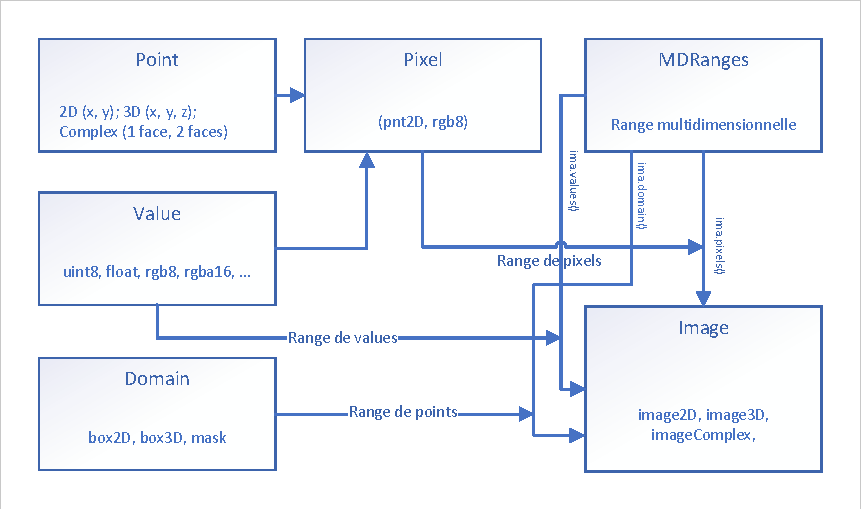
\includegraphics[width=.8\linewidth]{../figures/concepts/image_fr}
  \caption[]{Concept Image.}
  \label{resume:fig:concept.image}
\end{figure}

Enfin, ce chapitre introduit notre première contribution principale : une taxonomie complète relative au domaine du
traitement d'images. Nous introduisons d'abord des concepts fondamentaux tels que \emph{point}, \emph{pixel},
\emph{domaine} et \emph{image} (illustrés dans la~\cref{resume:fig:concept.image}). Nous motivons et introduisons
ensuite des concepts avancés liés aux images et aux différentes manières d'accéder aux données (parcours en avant,
renversé, indexation, accès direct à la mémoire tampon sous-jacente, \ ldots). En fin de compte, nous introduisons les
concepts liés aux notions gravitant autour du traitement d'images, telles que les \emph{éléments structurants}, les
\emph{voisinages} et les \emph{extensions} (gestion des bordures) qui sont nécessaires pour pouvoir travailler avec des
algorithmes locaux.

Le chapitre suivant utilise les concepts présentés pour introduire la deuxième contribution principale de cette thèse :
les \emph{vues d'image}.


\subsection*{Les Vues d'Image}


Cette notion de vues n'est pas nouvelle~\parencite{novak.1997.reuse} et est apparue naturellement en Traitement d'images
avec Milena~\parencite{geraud.2012.ipolmeeting,levillain.2010.icip} sous le nom de
\emph{morpher}~\parencite{levillain.2009.ismm, geraud.2012.hdr}. Il était toujours utile de pouvoir projeter une image à
travers un prisme qui pourrait extraire des informations spécifiques à son sujet sans avoir besoin de copier la mémoire
tampon des données sous-jacentes. Aujourd'hui (2020), le langage C++ (norme 20) introduit aussi ce mécanisme avec les
ranges~\parencite{niebler.2014.ranges} pour les \emph{collections non-propriétaires} (de leur mémoire). Il est nommé
\emph{vues} (view) et permet à l'utilisateur d'accéder au contenu d'une collection de données (vector, map) à travers un
prisme. Dans Pylene, nous avons décidé de nous aligner sur la nomenclature normalisé dans C++20 afin de ne pas dérouter
l'utilisateur. De cette façon, une vue \texttt{transform} dans le traitement d'images fait la même chose sur une image
que ce que la vue \texttt{transform} fait sur un conteneur (collection) dans la bibliothèque de ranges standard. Les
\emph{vues} présentent les propriétés suivantes : \emph{copie quasi gratuite}, \emph{non-propriétaire} (ne
\emph{possède} aucune mémoire tampon contenant des données), \emph{évaluation paresseuse} (l'accès à la valeur d'un
pixel peut nécessiter des calculs) et \emph{composable}. Lorsque les vues sont chaînées, le compilateur construit un
\emph{arbre d'expressions} (ou \emph{expression template} tel qu'utilisé dans de nombreuses bibliothèques de calcul
scientifique telles qu'Eigen~\parencite{guennebaud.2010.eigen}). Le compilateur connaît donc le type de la
composition finale et s'assure qu'il n'y ait pas de surcoût en performance à l'exécution (0-overhead). Tout d'abord nous
motivons l'utilisation des \emph{vues} dans le traitement d'images, ensuite nous présentons les principales vues
utilisées en traitement d'images. Puis, nous discutons de la façon dont les vues d'image diffèrent de celles
utilisées dans les ranges de C++ et leurs principales propriétés (en particulier comment elles conservent/suppriment les
propriétés de l'image parente) à travers un exemple concret : la gestion des bordures et des extensions. Enfin, nous
étudions les limites liées à ce design.

En traitement d'images, un algorithme s'écrit naïvement en prenant une ou plusieurs données d'entrée (parmi lesquelles
figurent la/les image(s) d'entrée), en effectuant un traitement sur ces données d'entrée puis en retournant les données
résultantes (ou une erreur). Prenons par exemple l'algorithme mélange alpha (alpha-blending) qui peut être implémenté en
C++ naïf comme suit :
\begin{minted}{C++}
  void blend_inplace(const uint8_t* ima1, uint8_t* ima2, float alpha,
  int width, int height, int stride1, int stride2) {
    for (int y = 0; y < height; ++y) {
      const uint8_t* iptr = ima1 + y * stride1;
      uint8_t* optr = ima2 + y * stride2;
      for (int x = 0; x < width; ++x)
        optr[x] = iptr[x] * alpha + optr[x] * (1-alpha);
    }
  }
\end{minted}

Ce code a plusieurs défauts. Il fait des hypothèses fortes sur les images d'entrée : la contiguïté de ses données dans
sa mémoire tampon et sa forme (2D). Supposons que notre utilisateur veuille maintenant restreindre l'algorithme à une
région spécifique à l'intérieur de l'image. Le mainteneur devrait alors fournir une surcharge de fonction pour
l'algorithme avec un argument d'entrée supplémentaire correspondant à la région d'intérêt. Supposons que l'utilisateur
veuille ensuite prendre en charge la manipulation d'images 3D. Le mainteneur devrait également fournir deux surcharges
de fonction supplémentaires avec un argument de \emph{pas} supplémentaire (un pour l'algorithme de base, un l'algorithme
prenant en compte une région d'intérêt). Supposons finalement que l'utilisateur souhaite uniquement manipuler le canal
de couleur rouge. Alors le mainteneur doit le prendre en charge et ajouter des surcharges de fonctions supplémentaires
pour chaque canal et/ou type de couleurs gérés. La complexité augmente grandement pour chaque point de customisation que
le mainteneur souhaite offrir à l'utilisateur. Bien sûr, il est possible d'empêcher la duplication de code grâce à une
utilisation intelligente des techniques d'ingénierie informatique (factorisation de code, etc.) mais la complexité
fuiterait toujours à travers l'API dans une certaine mesure. C'est ainsi que l'autre solution consiste à permettre à
l'utilisateur d'effectuer ces restrictions en amont de l'algorithme de manière transparente afin que l'algorithme en
aval soit facile à écrire, comprendre et maintenir. Pour y parvenir, nous devons augmenter le niveau d'abstraction
autour des images d'un niveau afin que nous puissions travailler directement au niveau de l'image. L'algorithme de
mélange alpha (alpha-blending) s'écrirait alors comme indiqué dans la~\cref{resume:fig:view.alphablend}.

\begin{figure}[htbp]
  \centering
  \includestandalone[mode=image, scale=0.7]{../figures/alphablend}

  \caption[]{Algorithme mélange alpha (alpha-blending) écrit au niveau de l'image.}
  \label{resume:fig:view.alphablend}
\end{figure}

Cette façon d'exprimer un algorithme est obtenue en introduisant des \emph{vues} dans le traitement d'images. Une image
est maintenant une vue et peut être restreinte/projetée/manipulée selon les besoins de l'utilisateur avant de la
transmettre à un algorithme. Même l'algorithme de mélange alpha (alpha-blending) peut entièrement être réécrit en termes
de vues, comme montré dans la~\cref{resume:fig:new.alphablend}.

\begin{figure}[htbp]
  \centering
  \begin{minipage}[b]{5.5cm}
    \includestandalone[mode=image, scale=1.0]{../figures/view_ast2}
  \end{minipage}
  \begin{minipage}[b]{5.5cm}
    \begin{minted}{c++}
    auto alphablend =
      [](auto ima1, auto ima2, float alpha) {
        return alpha * ima1 + (1 - alpha) * ima2;
      };
    \end{minted}
    \bigskip
    \bigskip
    \bigskip
  \end{minipage}
  \caption[]{Mélange alpha (alpha-blending), implémentation générique avec les \emph{views}, et son arbre
             d'expressions.}
  \label{resume:fig:new.alphablend}
\end{figure}

Être capable d'effectuer de puissantes manipulations sur les images avant de les passer aux algorithmes annule
complètement le problème initial qui consiste à avoir plusieurs surcharges de fonctions pour un même algorithme tout en
maintenant et en documentant tous les arguments optionnels associés. En effet, pour effectuer la transformation de
mélange alpha (alpha-blending) sur l'image d'entrée, tout ce que l'utilisateur doit faire est :
\begin{minted}{C++}
  auto ima1, ima2 = /* ... */;
  auto ima_blended = alphablend(ima1, ima2, 0.2);
\end{minted}
Si l'utilisateur souhaite restreindre la région à mélanger ou le canal de couleur sur lequel travailler, il lui suffit
d'écrire la modification suivante :
\begin{minted}{C++}
  auto roi = /* ... */;
  auto blended_roi = alphablend(view::clip(ima1, roi), view::clip(ima2, roi), 0.2);
  auto blended_red = alphablend(view::red(ima1), view::red(ima2), 0.2);
\end{minted}
La restriction est faite en amont de l'algorithme et propagée en aval sans augmenter la complexité du code. De cette
façon, les vues augmentent considérablement ce que l'utilisateur peut faire, tout en écrivant moins de code.

\begin{figure}[htbp]
  \centering
  \includegraphics[scale=0.7]{../figures/pipeline_fr}
  \caption[]{Exemple d'une pipeline de traitement d'images simple.}
  \label{resume:fig:view.pipeline}
\end{figure}

Dans ce chapitre, nous voyons que \emph{les vues sont composables}. L'une des caractéristiques les plus importantes dans
la conception d'une pipeline (généralement, en génie logiciel) est la \emph{composition d'objets}. Elle permet de
composer des blocs simples entre eux pour former des blocs complexes. Ces blocs complexes peuvent alors être gérés comme
s'il s'agissait à nouveau de blocs simples. Dans la~\cref{resume:fig:view.pipeline}, nous avons 3 opérateurs de traitement d'image simples \emph{Image}~\(\rightarrow\)~\emph{Image} (la conversion en niveaux de gris, la sous-quantification et la dilatation). Comme indiqué dans la~\cref{resume:fig:view.comp}, la composition des algorithmes considérerait ces 3 opérateurs simples comme un seul opérateur complexe \emph{Image}~\(\rightarrow\)~\emph{Image} qui pourrait ensuite être utilisé dans une pipeline de traitement d'image encore plus complexe. Tout comme les algorithmes, les vues d'image sont composables. Par exemple, une vue de la vue d'une image reste toujours une image. Dans la~\cref{resume:fig:view.comp}, nous composons l'image d'entrée avec une vue de transformation en niveaux de gris puis avec une vue de sous-quantification qui alimente enfin l'algorithme de dilatation.

\begin{figure}[htbp]
  \centering
  \includegraphics[scale=0.7]{../figures/composition_fr}
  \caption[]{Exemple d'une pipeline de traitement d'images simple illustrant la différence entre la composition
    d'algorithmes et la composition de vues d'image.}
  \label{resume:fig:view.comp}
\end{figure}

\FIXME{Aussi}, les \emph{vues améliorent l'utilisabilité}. Le code pour composer des images dans la~\cref{resume:fig:view.comp}
est presque aussi simple que :

\begin{minted}{c++}
  auto input = imread(...);
  auto A = transform(input, [](rgb16 x) -> float {
    return (x.r + x.g + x.b) / 3.f; }; );
  auto MyComplexImage = transform(A, [](float x)
    -> uint8_t { return (x / 256 + .5f); }; );
\end{minted}

Les personnes familiarisées avec la programmation fonctionnelle peuvent remarquer des similitudes avec ces langages où
\emph{transform} (\emph{map}) et \emph{filter} sont des opérateurs de séquence. Les vues utilisent le paradigme
fonctionnel et sont créées par des fonctions qui prennent une fonction en argument : l'opérateur ou le prédicat à
appliquer pour chaque pixel ; nous n'itérons pas à la main sur les pixels de l'image.

De plus, les \emph{vues améliorent la ré-utilisabilité}. Les extraits de code ci-dessus sont simples, mais peu
réutilisables. Cependant, suivant le paradigme de la programmation fonctionnelle, il est assez facile de définir de
nouvelles vues, car certains adaptateurs d'image peuvent être considérés comme des \emph{fonctions d'ordre supérieur}
pour lesquelles nous pouvons lier certains paramètres, comme nous le ferions avec la technique de
currying~\parencite{hanus.1995.curry}. Dans la~\cref{resume:fig:view.highorder}, nous montrons comment la primitive
\emph{transform} peut être utilisée pour créer une vue additionnant deux images, une vue effectuant la conversion en
niveaux de gris et une vue effectuant une sous-quantification. Ces vues de base, réutilisable par la suite\footnote{Ces
fonctions auraient pu être écrites de manière plus générique pour plus de ré-utilisabilité, mais ce n'est pas le but
ici.}, sont ensuite chaînées ensembles pour créere image complexe.

\begin{figure}
  \begin{minted}{c++}
auto operator+(Image A, Image B) {
  return transform(A, B, std::plus<>());
}
auto togray = [](Image A) { return transform(A, [](auto x)
  { return (x.r + x.g + x.b) / 3.f; };)
};
auto subquantize16to8b = [](Image A) { return transform(A,
  [](float x) { return uint8_t(x / 256 +.5f); });
};

auto input = imread(...);
auto MyComplexImage = subquantize16to8b(togray(A));
  \end{minted}

  \caption[]{Utilisation de fonctions d'ordre supérieur pour créer des opérateurs de vues personnalisées.}
  \label{resume:fig:view.highorder}
\end{figure}

Par ailleurs, \emph{les vues sont calculées paresseusement}. L'opération étant enregistrée dans la vue d'image, ce
nouveau type d'image permet de mélanger des types d'image fondamentaux avec des algorithmes. Dans
la~\cref{resume:fig:view.highorder}, la création de vues n'implique aucun calcul en soi, mais retarde plutôt le calcul
jusqu'à ce que l'expression \texttt{v(p)} soit invoqué. Parce que les vues peuvent être composées, l'évaluation peut
être assez retardée. Les adaptateurs d'image sont des \emph{expressions template}~\parencite{veldhuizen.1995.expression,
veldhuizen.2000.blitz} car ils enregistrent les \emph{expressions} utilisées pour générer l'image en tant que paramètre
template. Une vue représente en fait un arbre d'expressions (\cref{resume:fig:new.alphablend}).

\emph{Les vues sont efficaces}. Avec un design classique, chaque opération de la pipeline est implémentée << par
elle-même >>. Chaque opération nécessite que de la mémoire lui soit allouée pour l'image de sortie et, également, chaque
opération nécessite que l'image soit entièrement parcourue. Ce design est simple, flexible, composable, mais n'est pas
efficace ni terme en mémoire ni performance de calcul. Avec l'évaluation paresseuse, l'image n'est parcourue qu'une
seule fois (lorsque la dilatation est appliquée), ce qui a deux avantages. Premièrement, il n'y a pas d'images
intermédiaires, ce qui est très efficient en termes de mémoire. Deuxièmement, la traversée de l'image est plus rapide
grâce à une meilleure utilisation du cache mémoire et effectue une traversée sélective optimale. En effet, dans notre
exemple (\cref{resume:fig:view.pipeline}), le traitement d'un pixel RVB16 de l'algorithme de dilatation le convertit
directement en niveaux de gris, puis le sous-quantifie en 8 bits, et enfin le rend disponible pour l'algorithme de
dilatation. Il agit \emph{comme si} nous écrivions un opérateur optimal qui combinerait toutes ces opérations. Cette
approche est quelque peu liée aux opérations de fusion du noyau disponibles dans certains HPC
spécifications~\parencite{openvx.2019}, mais la fusion de vues est optimisée par le compilateur C++
seulement~\parencite{brown.2018.ranges}. L'aspect sélectif intervient lorsqu'une région d'intérêt intervient dans la
pipeline de traitement. En effet, l'intégralité de la pipeline n'est alors exécuté que sur la région d'intérêt et ce
même si cette sélection n'est faite qu'à la toute fin de la pipeline de traitement.

Enfin, les \emph{vues améliorent la productivité}. Tous les algorithmes de traitement d'images fonctionnant pixel par
pixel peuvent (et doivent) être réécrits intuitivement en utilisant une vue en une seule ligne. Les vues
\emph{transform} sont la clé permettant ce point. Cela implique qu'il existe un nouveau niveau d'abstraction disponible
pour le traiteur d'image lors du prototypage de son algorithme. Le temps passé à la mise en \oe{}uvre des
fonctionnalités est réduite, donc le temps de la boucle de rétroaction est également réduit. Cela amène naturellement un
gain de productivité au traiteur d'image.


\subsection*{Un pont entre le monde statique et le monde dynamique}


Dans le monde de la programmation, il existe trois grandes familles de langage de
programmation~\parencite{prechelt.2000.comparison}. Il existe (i) les langages de programmation \emph{compilés}, tels
que C, C++, Rust ou Go, (ii) les langages de programmation \emph{interprétés}, tels que Python, PHP, Lisp ou Javascript,
et (iii) les langages de programmation hybrides, tels que Java ou C\#. Ces derniers ont une passe de compilation rapide
qui compile le code source dans un bytecode intermédiaire. Ensuite, ce bytecode est interprété via un interpréteur sur
une machine hôte.

\begin{figure}[htbp]
  \centering
  \includegraphics[width=.6\linewidth]{../figures/type-erased_buffer_fr}
  \caption[]{Pont entre Python et C++ grâce à Pybind11 et un effacement de type en C++.}
  \label{resume:fig:type-erased.buffer}
\end{figure}

Dans ce chapitre, nous concevons de nombreuses solutions pour résoudre plusieurs types de problèmes liés au pont entre
le monde statique et le monde dynamique. Nous présentons notre solution hybride capable de rendre disponible notre
bibliothèque générique C++ (statique) à partir de Python (dynamique). Nous discutons à propos des différentes façons de
réaliser ce pont, leurs avantages et leurs inconvénients. Aussi, nous introduisons une nouvelle couche d'abstraction, le
value-set, qui est un moyen standard de manipuler les valeurs sous-jacentes d'une image, utilisable lors de la mise en
\oe{}uvre d'algorithmes de traitement d'images. Cette nouvelle couche d'abstraction permet notamment à l'utilisateur
d'injecter du code côté Python dans des routines C++ déjà compilées. Cependant, superposer une couche d'abstraction
après l'autre, ou même appeler du code Python entraine forcément un coût du côté des performances. C'est pourquoi nous
avons réalisé un benchmark pour exposer clairement le coût de nos différentes solutions. Ce benchmark compare les quatre
versions de notre algorithme d'étirement (stretch) dont l'implémentation et l'utilisation sont détaillées dans le
chapitre. Le résultat est affiché dans le~\cref{resume:table:static.dynamic.perfs}.

\begin{table}[htbp]
  \footnotesize
  \centering
  \begin{tabular}{l|ccc}
    \toprule
    Type de Dispatch &
    Compute Time     &
    \(\Delta{}\)Compute Time
    \\ \midrule Value-set natif avec des types de valeurs C++ natifs (baseline)
                     & \(0.0093s\) & \(0\)                        \\
    \makecell[l]{Value-set comprenant un appel virtuel avec       \\ des types de valeurs C++ natifs}      &
    \(0.1213s\)      &
    \(\times 13\)
    \\
    \makecell[l]{Value-set comprenant un appel virtuel avec       \\ des types de valeurs C++ cachées par un effacement de type} &
    \(1.0738s\)      &
    \(\times 115\)
    \\
    \makecell[l]{Value-set injecté depuis Python avec Python avec \\ des types de valeurs C++ natifs} &
    \(21.5444s\)     &
    \(\times 2316\)
    \\
    \bottomrule
  \end{tabular}
  \caption[]{Benchmarks de toutes nos version de l'algorithme d'étirement (stretch).}
  \label{resume:table:static.dynamic.perfs}
\end{table}

Ce benchmark montre que chaque fois qu'une couche d'abstraction est ajoutée au-dessus de baseline, l'utilisateur doit
s'attendre à un facteur \(10\times\) impactant les performances de son code. De plus, appeler du code Python est
immensément plus lent (\(2300\times\) !) que la baseline. Cela renouvelle l'intérêt de recompiler la bibliothèque C++
générique avec un type paramétrique supplémentaire connu plutôt que de l'injecter depuis Python, surtout pour du code
qui met longtemps à s'exécuter. Pouvoir injecter du code Python facilite le prototypage et augmenter la vitesse à
laquelle l'utilisateur peut écrire son code. Cependant, le benchmark montre que ce n'est pas une solution viable une
fois que le prototype doit être déployé dans un environnement de production.

\paragraph{Continuité : Solutions basées sur le JIT, avantages et inconvénients}

Notre solution hybride a certainement des avantages, mais l'énorme inconvénient est la lenteur pour injecter nos propres
types depuis Python. Il existe une autre solution que cette thèse n'a pas eu l'occasion d'approfondir. Cette solution
est basée sur une technologie connue : la compilation Just-In-Time (JIT) qui a été illustrée précédemment
in~\cref{resume:fig:static.dynamic.dynamic.pipeline} (et qui elle-même repose sur la notion de programmation
générative~\parencite{czarnecki.2000.generative}). Des bibliothèques telles que AsmJit~\parencite{kobalicek.2011.asmjit}
sont capables d'émettre du code machine directement en effectuant un appel depuis du code C++. En effet, c'est une
technologie déjà utilisée par les langages interprétés tels que Java ou PHP pour générer à la volée du code machine
natif et optimisé pour la section du code source qui est considéré comme << chaud >> par l'interpréteur. Un code source
est << chaud >> lorsqu'il est beaucoup exécuté : l'utilisateur final gagnerait beaucoup à payer le temps de compilation
une fois pour que ce code soit exécuté plus rapidement plusieurs fois par la suite. Appliquer cette solution à notre
problématique signifierait que l'utilisateur devrait être capable de compiler du code machine natif à partir du code C++
générique en injectant le type demandé, en tant que paramètre template, lorsqu'il est utilisé. Une telle opération
déplace fortement une charge sur l'utilisateur (compilation), et il est bien connu que compiler du code C++ est
notoirement \emph{compliqué} et \emph{lent}. De plus, la bibliothèque doit être capable de générer automatiquement
l'interface la liant au Python une fois le code C++ compilé. Il existe plusieurs solutions pour arriver à nos fins.

\begin{figure}[htbp]
  \centering
  \includegraphics[width=.6\linewidth]{../figures/dynamic_pipeline_fr}
  \caption{Language interpreté: diagramme d'exécution}
  \label{resume:fig:static.dynamic.dynamic.pipeline}
\end{figure}

La première solution consiste basiquement à faire des appels système aux compilateurs pour réellement \emph{compiler} le
code C++ une fois que le/les types template sont connus et explicitement instanciés dans le code source. Cette solution
nécessite une génération de code minutieuse et que l'utilisateur possède un compilateur fonctionnel sur son ordinateur.
De plus, l'utilisateur doit résoudre toutes les dépendances de la bibliothèque, comme \emph{freeimage} pour les
entrées/sorties, etc. Cette solution a été conçue dans la bibliothèque VCSN~\parencite{demaille.2013.vcsn}. En effet, à
chaque fois que l'utilisateur déclare un nouvel automate dans son notebook Jupyter, le code source correspondant est
compilé en arrière-plan puis est mis en cache. C'est une solution très périlleuse à mettre en place lorsque
l'environnement d'exécution final (OS, logiciels installés) n'est pas bien connu à l'avance. De nos jours, le problème
peut être moindre, cependant, il nécessite toujours de maintenir à la fois la bibliothèque et la solution de conteneur
pour l'utiliser (Docker).

La deuxième solution est d'utiliser Cython~\parencite{behnel.2010.cython}. C'est une infrastructure de transpilation qui
transforme un code source Python directement dans du code source du langage C afin qu'il puisse être compilé par un
compilateur C standard simplement en linkant contre l'API Python/C. Cela supprime la charge d'écrire la routine de
génération de code minutieuse, les appels système au compilateur C++ et supprime le besoin de résoudre toutes les
dépendances. Cette infrastructure s'occupe de tout pour l'utilisateur. De plus, en le transpilant en code C, la
compilation sera plus rapide, car un compilateur C est plus rapide qu'un compilateur C++. Cython prend même en charge
les template C++~\parencite{behnel.2022.cython-template} qui sont obligatoires pour notre cas d'utilisation.

La troisième solution consiste à s'appuyer sur des projets récents qui reposent tous sur l'infrastructure LLVM. Nous
pouvons notamment citer AutoWIG~\parencite{fernique.2018.autowig}, Cppyy~\parencite{wimtlplavrijsen.2016.cppyy},
Xeus-cling~\parencite{quantstack.2021.xeus-cling} et Pythran~\parencite{guelton.2015.pythran}. AutoWIG a du code <<
maison >> basé sur LLVM/Clang pour analyser le code C++ afin de générer et compiler une interface Python via Swig à
l'aide du moteur de template Mako. AutoWIG, couplé à Cython permettrait à l'utilisateur, par exemple, de générer du code
C lié à une structure Python personnalisée. Ensuite, un simple appel à AutoWIG analysera le code C et l'injectera dans
la bibliothèque C++ pour générer l'interface utilisable par l'utilisateur. En ce qui concerne Cppyy, il est basé sur
LLVM/Cling, un interpréteur C++, et peut interpréter directement du code C++ à partir d'une chaîne de caractère Python.
Cela permet d'injecter facilement des types personnalisés, qu'ils soient dans du code Python (transpilé avec Cython) ou
du code C++ (directement interprété par Cling). Ensuite, l'infrastructure génère l'interface utilisable à partir de la
bibliothèque C++ générique pour le type injecté demandé. Xeus-cling est un noyau Jupyter prêt à l'emploi permettant
l'utilisation du code C++ directement à partir d'un notebook. Cela permet de contourner complètement le besoin d'avoir
une interface avec Python et permet à l'utilisateur d'utiliser la bibliothèque depuis un notebook comme s'il s'agissait
une bibliothèque Python. Enfin, Pythran est un compilateur << avancé >> pour un sous-ensemble du langage Python, axé sur
le calcul scientifique. Il prend un code Python annoté avec quelques descriptions dans son interface et le transforme en
un module Python natif avec la même interface, mais en espérant qu'il soit plus rapide. Pythran tire parti du
multic\oe{}ur et des instructions SIMD pour transformer son sous-ensemble du langage Python en code C++ fortement
générique instancié pour des types optimisés bien particuliers. Toutes ces infrastructures, cependant, ont un coût élevé
en termes de taille de binaire. En effet, un compilateur C++ n'est pas petit et l'embarquer avec la bibliothèque de
traitement d'images peut facilement avoir un impact considérable sur la taille du binaire final. Sans l'infrastructure
LLVM, le binaire peut peser environ 3 Mo. Avec l'infrastructure LLVM, le poids du binaire devient au strict minimum 50
Mo. De plus, ces solutions peuvent ne pas être immédiatement plus rapides. En effet, lors du prototypage et des
multiples aller-retour avec une variété de types, l'utilisateur peut ne pas être patient et attendre les longs temps de
compilations à chaque fois qu'il teste avec une nouvelle itération de son travaille. Malgré cela, ces solutions offrent
d'excellentes voies de recherche pour l'avenir et l'auteur est impatient de les explorer.


\subsection*{Conclusion}


Le travail présenté dans cette thèse par l'auteur suit un arc narratif très clair. L'accent a d'abord été mis sur la
présentation de ce qu'est la notion de programmation générique (généricité), son histoire et comment chacun(e) peut la
comprendre, notamment dans sa vie de tous les jours, et en particulier lorsqu'elle est appliquée au traitement d'images.
La généricité est une notion vieille de 4 décennies qui a évolué et trouvé une utilisation dans des domaines très
modernes de notre société. En effet, Le traitement d'images est largement utilisé pour construire des applications
utilisées dans le monde entier. Cependant, il a été démontré à quel point il peut être difficile de mettre en \oe{}uvre
des solutions reposant sur la généricité. En effet, il existe une règle de trois liant généricité, performance et
facilité d'utilisation. La règle stipule qu'on ne peut avoir que deux de ces notions qu'en sacrifiant le troisième. Si
l'on veut être générique et efficace, alors la solution naïve sera très complexe à utiliser avec beaucoup de paramètres.
Si l'on veut qu'une solution soit générique et facile à utiliser, alors elle ne sera pas très efficace par défaut.
Enfin, si l'on veut une solution simple d'utilisation et efficace alors elle ne sera pas très générique. Dans cette
thèse, nous essayons de démontrer comment briser cette règle, et ce, en trois étapes.

La première étape, illustrée dans le chapitre \emph{Taxonomy for Image Processing}, a consisté à faire un inventaire des
types et familles d'images ainsi que des différents algorithmes de traitement d'images. L'objectif a été de produire une
taxonomie complète des types (pixel, image, éléments structurants, \ldots) et algorithmes (locaux, globaux, \ldots) liés
au traitement d'images afin de pouvoir extraire les Concepts (au sens Concepts C++). Cette première étape délimite le
périmètre de ce que l'auteur englobe dans la notion de \emph{généricité}. \`{A} partir de ce point de départ, il devient
plus facile d'écrire des algorithmes de traitement d'images, juste en en s'appuyant sur ces concepts. De plus,
différents concepts existent pour permettre aux développeurs d'algorithmes d'exploiter des propriétés (décomposabilité
des éléments structurants, contiguïté du buffer de l'image, \ldots) afin d'atteindre des performances maximales.

\`{A} ce stade, nous raisonnons encore à un niveau bas (pixel) ce qui génère le besoin de designer une couche
d'abstraction afin de permettre un prototypage rapide pour des opérations simples tout en garantissant une empreinte
mémoire très faible et proche de zéro impact sur les performances. Pour cette raison, nous étendons le concept de
\emph{vues} du standard C++ (2020) aux images et nous clarifions la notion de \emph{vue d'image}. Nous faisons également
le choix de conception d'avoir une image légère, peu coûteuses à copier (données partagées buffer) par défaut afin de
fusionner l'image concrète et les vues du point de vue de l'utilisateur. L'évaluation paresseuse, qui se produit
systématiquement lors de l'utilisation des vues permet un gain de performances lors du découpage d'images volumineuses.
Dans le cas où l'image est traitée dans son entièreté, nous sommes tout de même capable d'obtenir des performances très
satisfaisantes qui restent stables. Aussi, nous montrons, à travers des cas d'utilisation concrets tels que les
algorithmes fonctionnant pixel par pixel et la gestion des frontières, comment l'utilisation des vues simplifie
grandement la façon d'écrire des algorithmes de traitement d'images plus complexes et efficaces par défaut. Nous
montrons enfin les limites de cette approche, avec un accent particulier sur la vitesse de parcours d'une image, qui est
un cas d'utilisation obligatoire que nous devons maîtriser.

Enfin, dans cette thèse, nous avons porté notre attention sur la manière dont il est possible de distribuer ce logiciel
à la communauté des traiteurs d'image qui travaille principalement avec Python. Cette dernière contribution concentre
ses efforts sur la recherche de la meilleure façon de concevoir un pont statique (C++ template, temps de la compilation)
--- dynamique (notebook Jupyter Python, moment de l'exécution) pour apporter efficacement ces notions (concepts et vues)
au traiteur d'image. Cette dernière contribution explore ce dilemme et propose de l'aborder avec une solution hybride
dont le design et les motivations sont expliqués en profondeur. Cette solution hybride s'appuie sur la technique de
l'effacement de type qui offre une compatibilité les \emph{NumPy.array}~\parencite{harris.2020.numpy}. Ce type (effacé)
est alors capable de se convertir au sein d'un dispatcher de cardinalité \(n \times n\) (dimension et type sous-jacent)
dans un type C++ templaté concret optimisé. Cette solution explique aussi comment écrire très simplement le code << glue
>> permettant d'exposer en Python des algorithmes déjà existants (en C++) grâce à une mécanique de dispatch fortement
inspirée du standard C++ (\texttt{std::visit}, \texttt{std::variant}). Le but de cette solution est de regrouper en un
seul endroit dans le code tous les types supportés dans les dispatcher pour faciliter la maintenance ainsi qu'un travail
minimal exigé de la part de la personne qui implémente d'algorithmes pour les exposer au Python, tout cela en gardant
des performances natives. En effet, aucune copie superflue n'est effectuée grâce à \emph{pybind11} et son
\emph{type-caster}: uniquement une conversion est effectuée du type effacé vers le type natif. Tout le travail qui est
fait dans l'algorithme est effectué sur le type natif optimisé. Enfin, cette solution offre un moyen d'injecter des
types Python personnalis\'{e}s dans la bibliothèque C++ générique à des fins de prototypage, grâce à une nouvelle couche
d'abstraction, mais au prix de lourdes pertes de performance. L'inconvénient de cette solution est évidemment le
gonflement de la taille du binaire résultante qui explose de façon exponentielle avec le nombre de types pris en charge
multiplié par le nombre d'algorithmes multiplié par le nombre d'autres données supportées (éléments structurants, label
map, etc.)

Nous concluons cette thèse en proposant de nouvelles pistes de recherche autour du domaine de la compilation
Just-In-Time (JIT) pour améliorer encore le pont entre le monde statique et le monde dynamique. L'auteur pense que cette
piste mérite d'être explorée, surtout avec les outils existants déjà prometteurs (Xeus-cling, Cppyy, Cython, AutoWIG,
Pythran) afin de résoudre le problème de gonflement du binaire. En effet, nous ne devrions compiler que ce dont
l'utilisateur a besoin, mais le prix d'entrée peut être d'embarquer statiquement un interpréteur C++ (LLVM/cling ?) dans
son binaire, ce qui en soi le gonflerait grandement. Il peut être possible, cependant, de s'appuyer sur l'infrastructure
système de l'utilisateur pour que le mainteneur ne soit pas obligé de distribuer un interpréteur/compilateur C++ en même
temps que le binaire de sa bibliothèque de traitement d'images. Il s'agit encore d'un domaine de recherche nouveau et
l'auteur souhaiterait vivement l'approfondir pour étudier ce qu'il est possible de réaliser dès aujourd'hui avec ces
outils pour la communauté du traitement d'images.
